\documentclass[]{book}
\usepackage{lmodern}
\usepackage{amssymb,amsmath}
\usepackage{ifxetex,ifluatex}
\usepackage{fixltx2e} % provides \textsubscript
\ifnum 0\ifxetex 1\fi\ifluatex 1\fi=0 % if pdftex
  \usepackage[T1]{fontenc}
  \usepackage[utf8]{inputenc}
\else % if luatex or xelatex
  \ifxetex
    \usepackage{mathspec}
  \else
    \usepackage{fontspec}
  \fi
  \defaultfontfeatures{Ligatures=TeX,Scale=MatchLowercase}
\fi
% use upquote if available, for straight quotes in verbatim environments
\IfFileExists{upquote.sty}{\usepackage{upquote}}{}
% use microtype if available
\IfFileExists{microtype.sty}{%
\usepackage{microtype}
\UseMicrotypeSet[protrusion]{basicmath} % disable protrusion for tt fonts
}{}
\usepackage[margin=1in]{geometry}
\usepackage{hyperref}
\hypersetup{unicode=true,
            pdftitle={Distributed Machine Learning in R with Apache Spark},
            pdfauthor={Brandon M. Greenwell},
            pdfborder={0 0 0},
            breaklinks=true}
\urlstyle{same}  % don't use monospace font for urls
\usepackage{natbib}
\bibliographystyle{apalike}
\usepackage{color}
\usepackage{fancyvrb}
\newcommand{\VerbBar}{|}
\newcommand{\VERB}{\Verb[commandchars=\\\{\}]}
\DefineVerbatimEnvironment{Highlighting}{Verbatim}{commandchars=\\\{\}}
% Add ',fontsize=\small' for more characters per line
\usepackage{framed}
\definecolor{shadecolor}{RGB}{248,248,248}
\newenvironment{Shaded}{\begin{snugshade}}{\end{snugshade}}
\newcommand{\AlertTok}[1]{\textcolor[rgb]{0.94,0.16,0.16}{#1}}
\newcommand{\AnnotationTok}[1]{\textcolor[rgb]{0.56,0.35,0.01}{\textbf{\textit{#1}}}}
\newcommand{\AttributeTok}[1]{\textcolor[rgb]{0.77,0.63,0.00}{#1}}
\newcommand{\BaseNTok}[1]{\textcolor[rgb]{0.00,0.00,0.81}{#1}}
\newcommand{\BuiltInTok}[1]{#1}
\newcommand{\CharTok}[1]{\textcolor[rgb]{0.31,0.60,0.02}{#1}}
\newcommand{\CommentTok}[1]{\textcolor[rgb]{0.56,0.35,0.01}{\textit{#1}}}
\newcommand{\CommentVarTok}[1]{\textcolor[rgb]{0.56,0.35,0.01}{\textbf{\textit{#1}}}}
\newcommand{\ConstantTok}[1]{\textcolor[rgb]{0.00,0.00,0.00}{#1}}
\newcommand{\ControlFlowTok}[1]{\textcolor[rgb]{0.13,0.29,0.53}{\textbf{#1}}}
\newcommand{\DataTypeTok}[1]{\textcolor[rgb]{0.13,0.29,0.53}{#1}}
\newcommand{\DecValTok}[1]{\textcolor[rgb]{0.00,0.00,0.81}{#1}}
\newcommand{\DocumentationTok}[1]{\textcolor[rgb]{0.56,0.35,0.01}{\textbf{\textit{#1}}}}
\newcommand{\ErrorTok}[1]{\textcolor[rgb]{0.64,0.00,0.00}{\textbf{#1}}}
\newcommand{\ExtensionTok}[1]{#1}
\newcommand{\FloatTok}[1]{\textcolor[rgb]{0.00,0.00,0.81}{#1}}
\newcommand{\FunctionTok}[1]{\textcolor[rgb]{0.00,0.00,0.00}{#1}}
\newcommand{\ImportTok}[1]{#1}
\newcommand{\InformationTok}[1]{\textcolor[rgb]{0.56,0.35,0.01}{\textbf{\textit{#1}}}}
\newcommand{\KeywordTok}[1]{\textcolor[rgb]{0.13,0.29,0.53}{\textbf{#1}}}
\newcommand{\NormalTok}[1]{#1}
\newcommand{\OperatorTok}[1]{\textcolor[rgb]{0.81,0.36,0.00}{\textbf{#1}}}
\newcommand{\OtherTok}[1]{\textcolor[rgb]{0.56,0.35,0.01}{#1}}
\newcommand{\PreprocessorTok}[1]{\textcolor[rgb]{0.56,0.35,0.01}{\textit{#1}}}
\newcommand{\RegionMarkerTok}[1]{#1}
\newcommand{\SpecialCharTok}[1]{\textcolor[rgb]{0.00,0.00,0.00}{#1}}
\newcommand{\SpecialStringTok}[1]{\textcolor[rgb]{0.31,0.60,0.02}{#1}}
\newcommand{\StringTok}[1]{\textcolor[rgb]{0.31,0.60,0.02}{#1}}
\newcommand{\VariableTok}[1]{\textcolor[rgb]{0.00,0.00,0.00}{#1}}
\newcommand{\VerbatimStringTok}[1]{\textcolor[rgb]{0.31,0.60,0.02}{#1}}
\newcommand{\WarningTok}[1]{\textcolor[rgb]{0.56,0.35,0.01}{\textbf{\textit{#1}}}}
\usepackage{longtable,booktabs}
\usepackage{graphicx,grffile}
\makeatletter
\def\maxwidth{\ifdim\Gin@nat@width>\linewidth\linewidth\else\Gin@nat@width\fi}
\def\maxheight{\ifdim\Gin@nat@height>\textheight\textheight\else\Gin@nat@height\fi}
\makeatother
% Scale images if necessary, so that they will not overflow the page
% margins by default, and it is still possible to overwrite the defaults
% using explicit options in \includegraphics[width, height, ...]{}
\setkeys{Gin}{width=\maxwidth,height=\maxheight,keepaspectratio}
\IfFileExists{parskip.sty}{%
\usepackage{parskip}
}{% else
\setlength{\parindent}{0pt}
\setlength{\parskip}{6pt plus 2pt minus 1pt}
}
\setlength{\emergencystretch}{3em}  % prevent overfull lines
\providecommand{\tightlist}{%
  \setlength{\itemsep}{0pt}\setlength{\parskip}{0pt}}
\setcounter{secnumdepth}{5}
% Redefines (sub)paragraphs to behave more like sections
\ifx\paragraph\undefined\else
\let\oldparagraph\paragraph
\renewcommand{\paragraph}[1]{\oldparagraph{#1}\mbox{}}
\fi
\ifx\subparagraph\undefined\else
\let\oldsubparagraph\subparagraph
\renewcommand{\subparagraph}[1]{\oldsubparagraph{#1}\mbox{}}
\fi

%%% Use protect on footnotes to avoid problems with footnotes in titles
\let\rmarkdownfootnote\footnote%
\def\footnote{\protect\rmarkdownfootnote}

%%% Change title format to be more compact
\usepackage{titling}

% Create subtitle command for use in maketitle
\newcommand{\subtitle}[1]{
  \posttitle{
    \begin{center}\large#1\end{center}
    }
}

\setlength{\droptitle}{-2em}

  \title{Distributed Machine Learning in R with Apache Spark}
    \pretitle{\vspace{\droptitle}\centering\huge}
  \posttitle{\par}
  \subtitle{An Introduction to the sparklyr and rsparkling packages}
  \author{Brandon M. Greenwell}
    \preauthor{\centering\large\emph}
  \postauthor{\par}
      \predate{\centering\large\emph}
  \postdate{\par}
    \date{2018-08-01}

\usepackage{booktabs}

\usepackage{amsthm}
\newtheorem{theorem}{Theorem}[chapter]
\newtheorem{lemma}{Lemma}[chapter]
\theoremstyle{definition}
\newtheorem{definition}{Definition}[chapter]
\newtheorem{corollary}{Corollary}[chapter]
\newtheorem{proposition}{Proposition}[chapter]
\theoremstyle{definition}
\newtheorem{example}{Example}[chapter]
\theoremstyle{definition}
\newtheorem{exercise}{Exercise}[chapter]
\theoremstyle{remark}
\newtheorem*{remark}{Remark}
\newtheorem*{solution}{Solution}
\begin{document}
\maketitle

{
\setcounter{tocdepth}{1}
\tableofcontents
}
\hypertarget{preface}{%
\chapter*{Preface}\label{preface}}
\addcontentsline{toc}{chapter}{Preface}

This is a \emph{sample} book written in \textbf{Markdown}. You can use
anything that Pandoc's Markdown supports, e.g., a math equation
\(a^2 + b^2 = c^2\).

The \textbf{bookdown} package can be installed from CRAN or Github:

\begin{Shaded}
\begin{Highlighting}[]
\KeywordTok{install.packages}\NormalTok{(}\StringTok{"bookdown"}\NormalTok{)}
\CommentTok{# or the development version}
\CommentTok{# devtools::install_github("rstudio/bookdown")}
\end{Highlighting}
\end{Shaded}

Remember each Rmd file contains one and only one chapter, and a chapter
is defined by the first-level heading \texttt{\#}.

To compile this example to PDF, you need XeLaTeX. You are recommended to
install TinyTeX (which includes XeLaTeX):
\url{https://yihui.name/tinytex/}.

\hypertarget{part-part-i}{%
\part{Part I}\label{part-part-i}}

TBD.

\hypertarget{intro}{%
\chapter{Introduction to Apache Spark}\label{intro}}

\hypertarget{what-is-spark}{%
\section{What is Spark?}\label{what-is-spark}}

\begin{itemize}
\item
  Apache Spark (\url{https://spark.apache.org/}) is a unified analytics
  engine and cluster computing framework for large-scale data
  processing.
\item
  Does not use \emph{MapReduce} as an execution engine. Rather, Spark
  uses its own distributed runtime to execute work on a cluster.
\item
  It is designed to perform both batch processing (similar to MapReduce)
  and new workloads like streaming, interactive queries, and machine
  learning
\item
  Spark is closely integrated with \emph{Hadoop}, an open-source
  software framework for storing data and running applications on
  clusters.

  \begin{itemize}
  \item
    Spark can run on \emph{YARN}. This is the most convenient way to use
    Spark when you have an existing Hadoop cluster.
  \item
    Spark is compatible with Hadoop data (e.g., Spark works with Hadoop
    file formats and storage backends like \emph{parquet}).
  \item
    To be clear, you do not need Hadoop to run Spark, but you'll need
    some form of shared file system in order to run Spark on a cluster.
  \end{itemize}
\end{itemize}

\hypertarget{why-use-spark}{%
\section{Why use Spark?}\label{why-use-spark}}

\begin{itemize}
\item
  The most notable feature of Spark is its abaility to keep large
  working data sets in memory \emph{between jobs}.
\item
  There are two types of preccesses that benefit greatly from Sparks
  framework:

  \begin{itemize}
  \item
    Iterative algorithms.
  \item
    Interactive analysis.
  \end{itemize}
\item
  Spark uses a DAG (\emph{directed acyclic graph}) engine which can
  process arbitrary pipelines of operators that can be translated into a
  single job for the user.
\item
  Spark has a large community of experienced users.
\item
  Spark provides APIs to three languages: Scala, Java, Python, and R
  (through the \texttt{SparkR} package). An R interface to Apache Spark
  is also provided by the \texttt{sparklyr} package (which we'll
  primarily be using in this book). Spark also has several built-in SQL
  functions (Spark SQL).
\end{itemize}

\hypertarget{spark-dataframes}{%
\section{Spark DataFrames}\label{spark-dataframes}}

A Spark DataFrame is an optimized columnar data structure similar in
spirit to R/Pandas data frames. They can be constructed from a wide
variety of different including: CSV files, JSON files, parquet files,
Hive tables, external databases, data stored on HDFS, and many more. The
DataFrame API is available in Scala, Java, Python, and R. The
\texttt{sparklyr} package provides a \texttt{dplyr} backend that works
seemlessly with Spark DataFrames. There is also the concept of Spark
Datasets, but it will not be discussed in this book.

\hypertarget{apis-to-spark}{%
\section{APIs to Spark}\label{apis-to-spark}}

\hypertarget{scala}{%
\subsection{Scala}\label{scala}}

In a terminal, you can start a Spark session by typing

\begin{Shaded}
\begin{Highlighting}[]
\ExtensionTok{spark-shell}
\end{Highlighting}
\end{Shaded}

\hypertarget{java}{%
\subsection{Java}\label{java}}

\hypertarget{python}{%
\subsection{Python}\label{python}}

\hypertarget{r}{%
\subsection{R}\label{r}}

\begin{itemize}
\item
  The \texttt{sparklyr} package:

  \begin{itemize}
  \item
    Allows you to connect to Spark from R.
  \item
    Provides a complete \texttt{dplyr} backend.
  \item
    Provdes a SQL interface via the \texttt{DBI} package.
  \item
    Allows you to leverage Spark's distributed machine learning library
    (MLlib) from R.
  \item
    Allows you to leverage H2O' machine learning library
    (SparkingWater).
  \item
    Allows you to create extensions that call the full Spark API.
  \item
    Provides interfaces to Spark packages.
  \item
    For more information visit \url{http://spark.rstudio.com/}.
  \end{itemize}
\end{itemize}

\begin{figure}

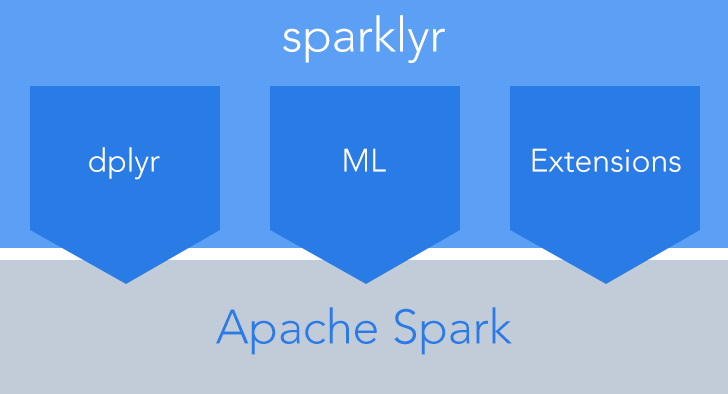
\includegraphics[width=0.7\linewidth]{illustrations/sparklyr-illustration} \hfill{}

\caption{Source: http://spark.rstudio.com/tools/readme/sparklyr-illustration.png.}\label{fig:sparklyr-illustration}
\end{figure}

\begin{itemize}
\tightlist
\item
  The \texttt{sparkR} package:
\end{itemize}

\hypertarget{spark-sql}{%
\subsection{Spark SQL}\label{spark-sql}}

\begin{itemize}
\item
  You can use of Spark SQL to execute SQL queries.
\item
  Spark SQL can also be used to read data from an existing \emph{Hive}
  installation.
\end{itemize}

\hypertarget{installing-spark}{%
\section{Installing Spark}\label{installing-spark}}

The easiest way to install spark is to use the
\texttt{sparklyr::spark\_install()} function. For example, to install
Spark version 2.3.0, use

\begin{Shaded}
\begin{Highlighting}[]
\NormalTok{sparklyr}\OperatorTok{::}\KeywordTok{spark_install}\NormalTok{(}
  \DataTypeTok{version =} \StringTok{"2.3.0"}\NormalTok{,}
  \DataTypeTok{hadoop_version =} \OtherTok{NULL}
\NormalTok{)}
\end{Highlighting}
\end{Shaded}

For details, see \texttt{?sparklyr::spark\_install}. To see what Spark
installations are available (along with there associated Hadoop
versions), use

\begin{Shaded}
\begin{Highlighting}[]
\KeywordTok{library}\NormalTok{(dplyr)}
\NormalTok{sparklyr}\OperatorTok{::}\KeywordTok{spark_available_versions}\NormalTok{(}\DataTypeTok{show_hadoop =} \OtherTok{TRUE}\NormalTok{) }\OperatorTok
\StringTok{  }\KeywordTok{arrange}\NormalTok{(}\KeywordTok{desc}\NormalTok{(spark), }\KeywordTok{desc}\NormalTok{(hadoop)) }\OperatorTok
\StringTok{  }\KeywordTok{slice}\NormalTok{(}\DecValTok{1}\OperatorTok{:}\DecValTok{5}\NormalTok{)  }\CommentTok{# only look at five latest versions}
\end{Highlighting}
\end{Shaded}

\begin{verbatim}
##   spark hadoop
## 1 2.3.0    2.7
## 2 2.3.0    2.6
## 3 2.2.1    2.7
## 4 2.2.1    2.6
## 5 2.2.0    2.7
\end{verbatim}

\hypertarget{linux}{%
\subsection{Linux}\label{linux}}

\hypertarget{macos}{%
\subsection{MacOS}\label{macos}}

\hypertarget{windows}{%
\subsection{Windows}\label{windows}}

\begin{itemize}
\tightlist
\item
  By a Unix machine 🤣.
\end{itemize}

\hypertarget{glossary-of-useful-terms}{%
\section{Glossary of useful terms}\label{glossary-of-useful-terms}}

\hypertarget{further-reading}{%
\section{Further reading}\label{further-reading}}

TBD.

\hypertarget{interfacing-r-with-spark}{%
\chapter{Interfacing R with Spark}\label{interfacing-r-with-spark}}

TBD.

\hypertarget{the-sparklyr-package}{%
\section{The sparklyr package}\label{the-sparklyr-package}}

\begin{Shaded}
\begin{Highlighting}[]
\KeywordTok{library}\NormalTok{(sparklyr)}
\NormalTok{sc <-}\StringTok{ }\KeywordTok{spark_connect}\NormalTok{(}\StringTok{"local[4]"}\NormalTok{)}
\KeywordTok{class}\NormalTok{(sc)}
\end{Highlighting}
\end{Shaded}

\begin{verbatim}
## [1] "spark_connection"       "spark_shell_connection"
## [3] "DBIConnection"
\end{verbatim}

\begin{Shaded}
\begin{Highlighting}[]
\NormalTok{pi_est <-}\StringTok{ }\ControlFlowTok{function}\NormalTok{() \{  }\CommentTok{# Monte-Carlo estimate of pi}
\NormalTok{  x <-}\StringTok{ }\KeywordTok{runif}\NormalTok{(}\DecValTok{100000}\NormalTok{)}
\NormalTok{  y <-}\StringTok{ }\KeywordTok{runif}\NormalTok{(}\DecValTok{100000}\NormalTok{)}
  \DecValTok{4} \OperatorTok{*}\StringTok{ }\KeywordTok{mean}\NormalTok{(x}\OperatorTok{^}\DecValTok{2} \OperatorTok{+}\StringTok{ }\NormalTok{y}\OperatorTok{^}\DecValTok{2} \OperatorTok{<}\StringTok{ }\DecValTok{1}\NormalTok{)}
\NormalTok{\}}

\KeywordTok{library}\NormalTok{(dplyr)}

\KeywordTok{sdf_len}\NormalTok{(sc, }\DataTypeTok{length =} \DecValTok{10}\NormalTok{, }\DataTypeTok{repartition =} \DecValTok{10}\NormalTok{) }\OperatorTok
\StringTok{  }\KeywordTok{spark_apply}\NormalTok{(pi_est) }\OperatorTok
\StringTok{  }\KeywordTok{summarize}\NormalTok{(}\StringTok{`}\DataTypeTok{Pi estimate}\StringTok{`}\NormalTok{ =}\StringTok{ }\KeywordTok{mean}\NormalTok{(id, }\DataTypeTok{na.rm =} \OtherTok{TRUE}\NormalTok{))}
\end{Highlighting}
\end{Shaded}

\begin{verbatim}
## # Source:   lazy query [?? x 1]
## # Database: spark_connection
##   `Pi estimate`
##           <dbl>
## 1          3.14
\end{verbatim}

\hypertarget{data-wrangling-in-spark-with-dplyr}{%
\section{Data wrangling in Spark with
dplyr}\label{data-wrangling-in-spark-with-dplyr}}

\hypertarget{the-sparkr-package}{%
\section{The sparkR package}\label{the-sparkr-package}}

\hypertarget{machine-learning-essentials}{%
\chapter{Machine Learning
Essentials}\label{machine-learning-essentials}}

TBD.

\hypertarget{part-part-ii}{%
\part{Part II}\label{part-part-ii}}

TBD.

\hypertarget{machine-learning-in-spark-via-mllib}{%
\chapter{Machine learning in Spark via
MLlib}\label{machine-learning-in-spark-via-mllib}}

TBD.

\hypertarget{machine-learning-in-spark-via-rsparkling}{%
\chapter{Machine learning in Spark via
rsparkling}\label{machine-learning-in-spark-via-rsparkling}}

TBD.

\bibliography{book.bib,packages.bib}


\end{document}
